\documentclass[11pt,a4paper]{article}
\usepackage[T1]{fontenc}
\usepackage[utf8]{inputenc}
\usepackage{lmodern}
\usepackage[a4paper,margin=2.5cm]{geometry}
\usepackage{amsmath,amssymb}
\usepackage{booktabs}
\usepackage{microtype}
\usepackage{graphicx}
\graphicspath{{figures/}}
\renewcommand{\thesection}{S\arabic{section}}
\renewcommand{\thetable}{S\arabic{table}}
\renewcommand{\thefigure}{S\arabic{figure}}
\newcommand{\Ind}{\ensuremath{\mathcal{I}}}

\title{\bfseries Supplementary Material\\[0.3em]
\large How Predictable Are Rare Precipitation Extremes?
A Calibration-Aware Assessment for London and Paris}
\author{Fankai Dong \and Olatunji Johnson}
\date{\today}

\begin{document}
\maketitle

\section{Results at the 99th-percentile threshold}
\label{sec:supp99}

The main paper analyses the $95$th-percentile index, which has $417$ extreme days
($287$ train, $130$ test). The $99$th-percentile index is far scarcer --- only
$137$ extreme days in thirty years ($101$ train, $36$ test) --- which precludes
the held-out intensity analysis (that requires extreme days in both train and
test across several splits). For completeness we report here the
\emph{occurrence} results of the simpler models at the $99$th percentile; the
deep Gaussian-process extreme-value hurdle, already dominated at the $95$th
percentile, is not re-run.

Table~\ref{tab:supp99} shows the bake-off (seed-averaged over three seeds, horizon
$h=1$), scored against climatology as in the main paper. The qualitative picture
matches the $95$th percentile but is weaker and noisier, as expected with a third
as many events:
\begin{itemize}
\item \textbf{Occurrence remains weakly predictable.} A plain calibrated logistic
regression with the ERA5 drivers beats climatology (Brier skill score
$+0.015$), improving on index history alone ($+0.001$); the gain again comes
chiefly from the convective-instability and circulation fields. Resolution
(informativeness) is positive but smaller than at the $95$th percentile
($0.36\times10^{-3}$ versus $0.83\times10^{-3}$).
\item \textbf{The distributional models fall below climatology.} With only $101$
training exceedances, the zero-inflated gamma and eGPD regressions are slightly
worse than climatology on the Brier score, and the zero-inflated log-normal is
again catastrophically miscalibrated --- echoing, more sharply, the main-paper
finding that the response distribution matters and that data scarcity penalises
the more flexible models.
\item \textbf{The tail is climatology-bound.} No model beats the climatological
tail on the threshold-weighted CRPS (all skill scores $\le 0$), and the scarce
exceedances do not support the held-out intensity test.
\end{itemize}

\begin{table}[h]
\centering
\caption{Bake-off at the $99$th-percentile threshold (London, $h=1$,
seed-averaged). Brier skill score (BSS) and threshold-weighted CRPS skill
(twCRPSS) are relative to climatology; positive is better. RES is the Brier
resolution ($\times10^3$). Climatology and a stationary peaks-over-threshold
model define the reference. Compare with Table~2 of the main paper
($95$th percentile).}
\label{tab:supp99}
\begin{tabular}{lccc}
\toprule
\textbf{Model} & \textbf{BSS} & \textbf{RES}$\times10^3$ & \textbf{twCRPSS} \\
\midrule
Climatology / stationary POT     & $0.000$  & $0.00$ & $0.000$ \\
Logistic (index history)         & $+0.001$ & $0.08$ & --- \\
Logistic ($+$ERA5)               & $\mathbf{+0.015}$ & $0.36$ & --- \\
ZI gamma ($+$ERA5)               & $-0.069$ & $0.20$ & $-0.130$ \\
ZI extended-GPD ($+$ERA5)        & $-0.048$ & $0.26$ & $-0.087$ \\
ZI log-normal ($+$ERA5)          & $-1.153$ & $0.25$ & $-4.827$ \\
\bottomrule
\end{tabular}
\end{table}

In short, the $99$th-percentile threshold tells the same story as the $95$th ---
weak but genuine occurrence predictability led by convective instability, a
climatology-bound tail, and a penalty on over-flexible models --- but with too
few events to support the intensity analysis or to add to the main conclusions.

\section{Paris: per-city diagnostic figures}
\label{sec:supp-paris}

The main paper shows the data, calibration, and horizon-decay diagnostics
(Figures~1, 2, and~4 there) for London as the representative city, while the
core comparative results --- the bake-off, the held-out intensity analysis, and
the unified hurdle --- are reported for both cities. For completeness we give the
Paris counterparts of the three single-city diagnostic figures here. They are
qualitatively identical to London: a zero-inflated, right-skewed, short-memory
index with a summer convective peak (Figure~\ref{fig:data-paris}); well-calibrated
exceedance probabilities from the simple logistic model, with the deep
Gaussian-process hurdle no better calibrated (Figure~\ref{fig:reliability-paris});
and occurrence skill decaying toward the prevalence floor with lead time while
conformal coverage stays at the nominal level (Figure~\ref{fig:horizon-paris}).
Paris differs from London only in having a higher extreme-day prevalence (a more
convective regime), consistent with its stronger predictability in the main text.

\begin{figure}[h]
\centering
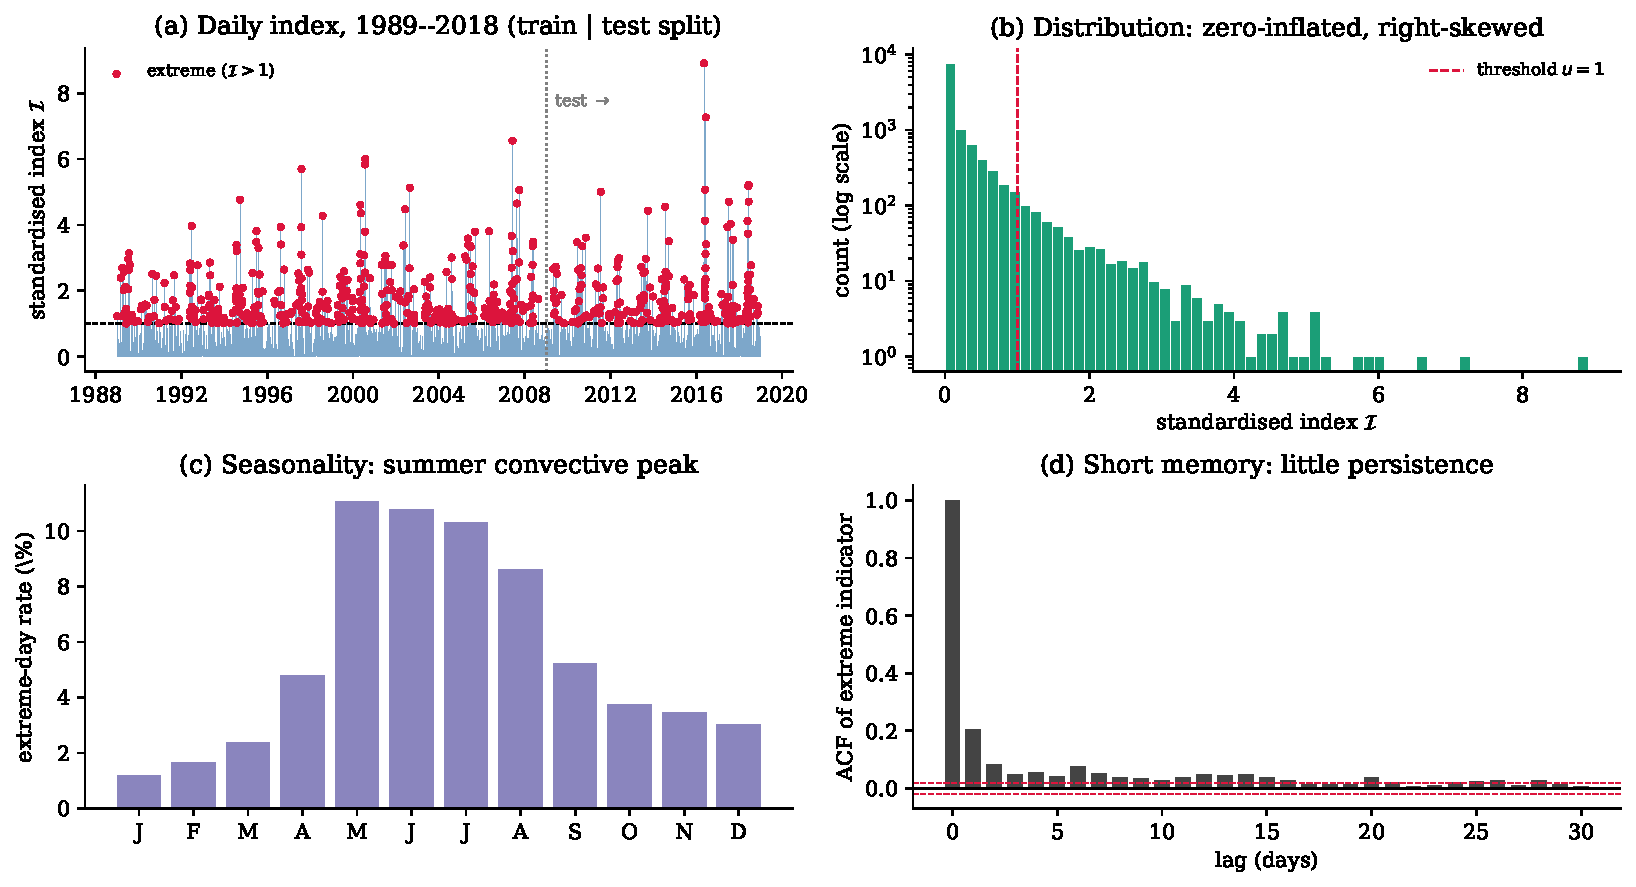
\includegraphics[width=\linewidth]{fig_data_paris}
\caption{Paris $95$th-percentile precipitation-extreme index (Paris counterpart of
Figure~1 in the main paper). \textbf{(a)} Daily index with extreme days
($\Ind>1$) and the train$\mid$test split; \textbf{(b)} zero-inflated, right-skewed
distribution; \textbf{(c)} summer-peaked seasonality of the extreme-day rate;
\textbf{(d)} short memory of the extreme indicator.}
\label{fig:data-paris}
\end{figure}

\begin{figure}[h]
\centering
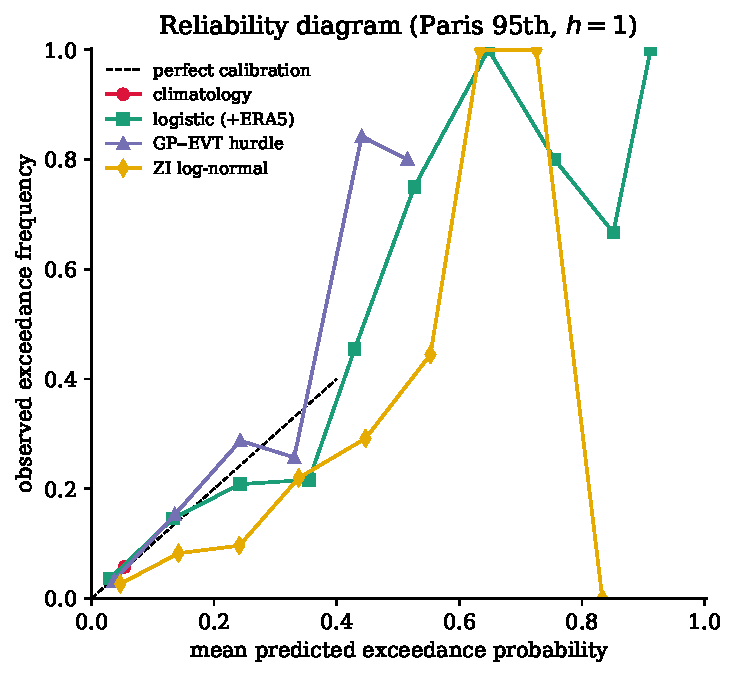
\includegraphics[width=0.62\linewidth]{fig_reliability_paris}
\caption{Reliability diagram for the Paris exceedance probability ($95$th, $h=1$;
Paris counterpart of Figure~2). The calibrated logistic model tracks the diagonal;
the deep Gaussian-process extreme-value hurdle is no better calibrated, mirroring
London.}
\label{fig:reliability-paris}
\end{figure}

\begin{figure}[h]
\centering
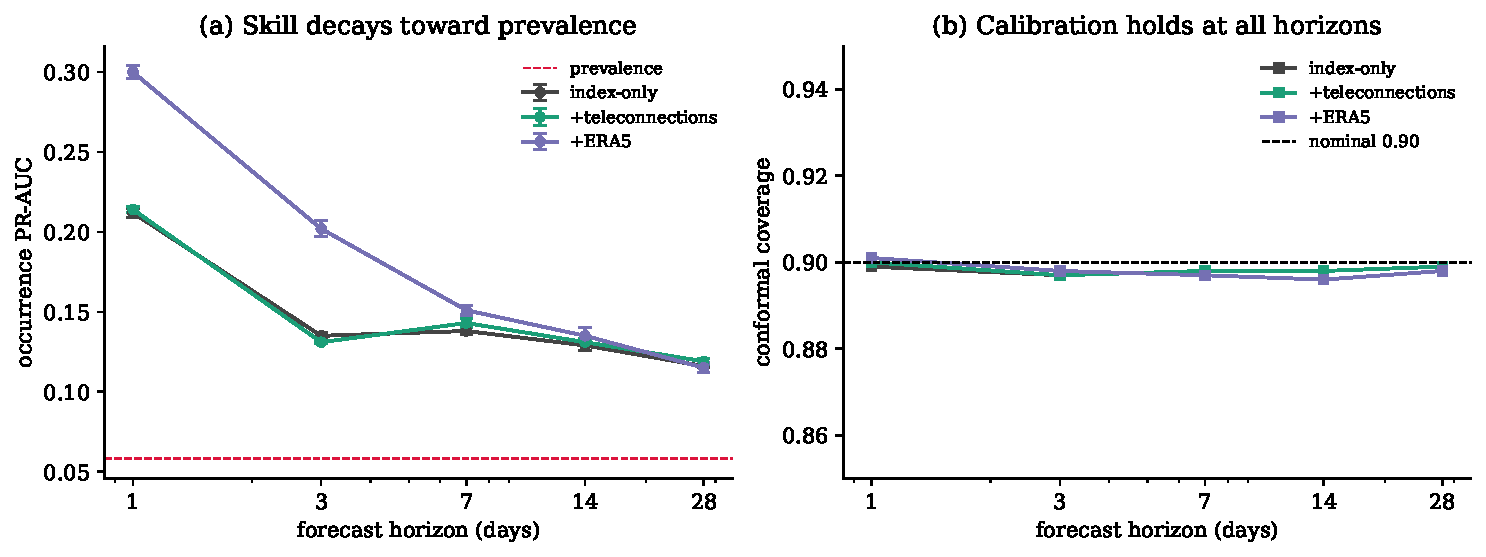
\includegraphics[width=\linewidth]{fig_horizon_paris}
\caption{Seed-averaged horizon sweep on the Paris $95$th-percentile index (Paris
counterpart of Figure~4). \textbf{(a)} Occurrence PR-AUC decays toward the
prevalence floor (dashed) as the horizon grows, with marginal driver gains;
\textbf{(b)} conformal coverage holds at the nominal $0.90$ across horizons and
predictor sets. Markers are means over three seeds.}
\label{fig:horizon-paris}
\end{figure}

\section{Feature importance and horizon-wise occurrence skill}
\label{sec:supp-features}

The main paper reports, in prose, that antecedent convective-instability and
circulation indices dominate the occurrence feature screen
(Section~5.3), and that occurrence skill decays with forecast horizon
(Section~5.6, Figure~4). We give both results here as tables, to make them
directly reproducible rather than only visually apparent.

Table~\ref{tab:supp-stability} shows the $15$ most frequently selected
features (of $d=49$; Section~3.3) under $L_1$-logistic stability selection
($200$ subsamples of $60\%$ of the training data, selection frequency = share
of subsamples in which a feature's coefficient is non-zero). The K-index of
convective instability (\texttt{kx\_mean}) and the most recent index lag
(\texttt{lag\_1}) are selected in essentially every subsample in both cities,
consistent with the main text; day-of-year seasonality, integrated
moisture/vapour-transport fields, the east--west mean-sea-level-pressure
gradient, and the NAO index also recur near the top of both lists.

\begin{table}[h]
\centering\small
\caption{Occurrence feature-importance: $L_1$-logistic stability-selection
frequency (top $15$ of $d=49$ features), $95$th percentile, $h=1$. Lags are
days; \texttt{exc30} is the $30$-day exceedance count; \texttt{sin/cos\_doy}
are seasonality harmonics; ERA5 fields are daily-mean unless marked
\texttt{max}.}
\label{tab:supp-stability}
\begin{tabular}{lc@{\qquad}lc}
\toprule
\multicolumn{2}{c}{\textbf{London}} & \multicolumn{2}{c}{\textbf{Paris}}\\
\textbf{Feature} & \textbf{Freq.} & \textbf{Feature} & \textbf{Freq.}\\
\midrule
lag\_1                  & $1.00$ & lag\_1                  & $1.00$ \\
IVT (mean)              & $0.99$ & lag\_6                  & $1.00$ \\
cos\_doy                & $0.99$ & K-index (mean)          & $1.00$ \\
sin\_doy                & $0.99$ & lag\_7                  & $0.99$ \\
K-index (mean)          & $0.98$ & IVT east (mean)         & $0.98$ \\
$500$hPa geopotential   & $0.98$ & MSLP grad.\ (E--W)      & $0.98$ \\
lag\_5                  & $0.95$ & lag\_5                  & $0.96$ \\
MSLP grad.\ (E--W)      & $0.93$ & cos\_doy                & $0.96$ \\
exc30                   & $0.91$ & NAO                     & $0.93$ \\
lag\_2                  & $0.88$ & lag\_14                 & $0.93$ \\
lag\_14                 & $0.83$ & exc30                   & $0.92$ \\
lag\_8                  & $0.82$ & lag\_3                  & $0.86$ \\
lag\_12                 & $0.82$ & MSLP grad.\ (N--S)      & $0.85$ \\
lag\_9                  & $0.82$ & lag\_12                 & $0.84$ \\
NAO                     & $0.81$ & lag\_2                  & $0.84$ \\
\bottomrule
\end{tabular}
\end{table}

Table~\ref{tab:supp-horizon} gives the Brier skill score (relative to
climatology) of the logistic $+$ERA5 occurrence model at each horizon of the
sweep $h\in\{1,3,7,14,28\}$ (single fit per horizon; RES is the Brier
resolution, $\times10^3$). This is the proper-score counterpart of the
discrimination-only (PR-AUC) horizon figure in the main paper and
Supplementary Figure~S3: in London, skill is effectively confined to $h=1$
and collapses toward zero by $h=3$; in Paris --- consistent with its larger,
more convective sample --- skill remains small but positive out to $h=28$,
though it decays steadily from its $h=1$ value.

\begin{table}[h]
\centering\small
\caption{Occurrence Brier skill score (BSS) by forecast horizon, logistic
$+$ERA5, $95$th percentile. RES ($\times10^3$) is the Brier resolution
(informativeness); climatology has BSS $=0$, RES $=0$ at every horizon by
construction.}
\label{tab:supp-horizon}
\begin{tabular}{lcccc}
\toprule
& \multicolumn{2}{c}{\textbf{London}} & \multicolumn{2}{c}{\textbf{Paris}}\\
\cmidrule(lr){2-3}\cmidrule(lr){4-5}
\textbf{Horizon $h$} & \textbf{BSS} & \textbf{RES} & \textbf{BSS} & \textbf{RES}\\
\midrule
$1$  & $+0.038$ & $0.829$ & $+0.117$ & $5.820$ \\
$3$  & $-0.000$ & $0.032$ & $+0.048$ & $2.435$ \\
$7$  & $-0.001$ & $0.047$ & $+0.032$ & $1.746$ \\
$14$ & $+0.002$ & $0.103$ & $+0.017$ & $0.708$ \\
$28$ & $+0.000$ & $0.009$ & $+0.015$ & $0.685$ \\
\bottomrule
\end{tabular}
\end{table}

\end{document}
